% Diese Zeile bitte -nicht- aendern.
\documentclass[course=erap]{aspdoc}

%%%%%%%%%%%%%%%%%%%%%%%%%%%%%%%%%
%% TODO: Ersetzen Sie in den folgenden Zeilen die entsprechenden -Texte-
%% mit den richtigen Werten.
\newcommand{\theGroup}{213} % Beispiel: 42
\newcommand{\theNumber}{A326} % Beispiel: A123
\author{Noah Schlenker \and Leon Baptist Kniffki \and Christian Krinitsin}
\date{Sommersemester 2023} % Beispiel: Wintersemester 2019/20
%%%%%%%%%%%%%%%%%%%%%%%%%%%%%%%%%

% Diese Zeile bitte -nicht- aendern.
\title{Gruppe \theGroup{} -- Abgabe zu Aufgabe \theNumber}

\usepackage{amsfonts}
\usepackage{amsmath}

\usepackage{subfig}

\begin{document}
\maketitle

\section{Einleitung} \label{sec:einleitung}
\begin{figure}[h] 
\centering
\subfloat[Lena: Photoshop-Output]{{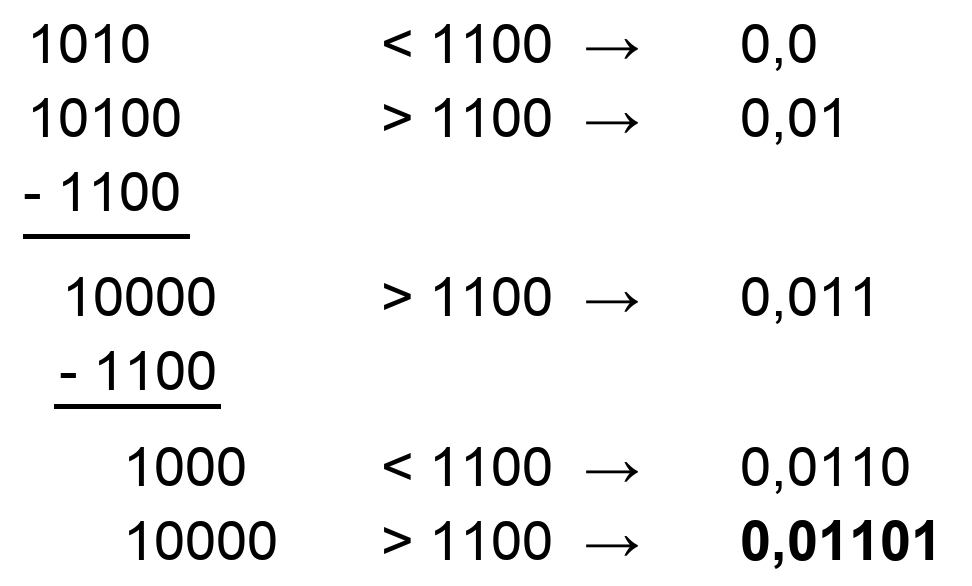
\includegraphics[scale=0.2]{graphiken/division-example.png} }}
\qquad
\subfloat[Lena: Code-Output]{{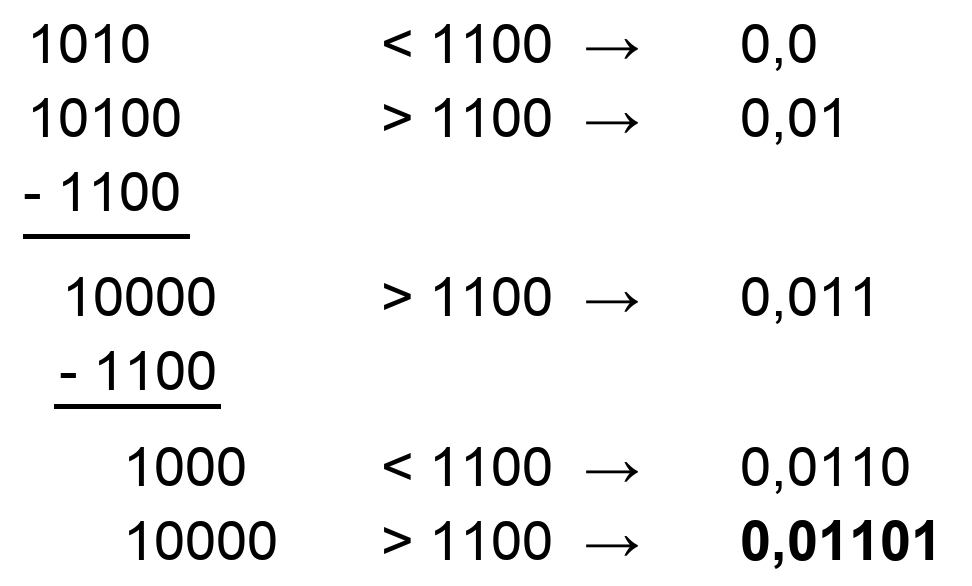
\includegraphics[scale=0.2]{graphiken/division-example.png} }}
\caption{Lena nach Graustufen und Weichzeichnen: Photoshop-Output (links) vs Code-Output (rechts)} 
\end{figure}

Schon im 1800 Jahrhundert v. Chr. beschäftigten sich die Babylonier mit der Quadratwurzel aus zwei. Mit $\tfrac {30547}{21600} = 1,\textbf{41421}2962\dots$ schafften sie eine Näherung, die nur
ab der fünften Nachkommastelle vom eigentlichen Ergebnis abweichte \cite{quadratwurzel_aus_2}. Außerdem schafften sie es, mit dem Beweis der Irrationalität der Wurzel aus 2, den ersten Beweis 
dieser Art aufzustellen, der abseits von Intuition, eine Überlegung und genaue Beweisführung erforderte \cite{lemonde_wurzel_2}. \par

Der Nutzen der bekanntesten irrationalen Zahl ist heute im Alltag weitreichend. So ist beim internationalen Standard für Papierformate das Seitenverhältnis stets $\frac{1}{\sqrt{2}}$ \cite{papierformat}. 
Dies hat zur Folge, dass beim Halbieren "des Blattes entlang der längeren Seite wieder ein Blatt im DIN-A-Format [...] entsteht" \cite{quadratwurzel_aus_2}. \par

In dieser Arbeit werden wir uns damit beschäftigen, wie man eine beliebige Anzahl an Nachkommastellen aus der Quadratwurzel aus zwei berechnet. Zu Beginn setzen wir uns dafür damit auseinander, 
wie man Zahlen mit beliebiger Größe speichern kann und arithmetische Operationen ausführen kann. Als nächstes wird beleuchtet, wie wir mithilfe von Matrizen und der schnellen Exponentiation
an den Wert von $\sqrt{2}$ approximieren. Es wird die Genauigkeit der Endergebnisse erläutert und zum Schluss die Performanz des Programms mithilfe von Vergleichsimplementierungen bewertet.

\section{Lösungsansatz} \label{sec:loesungsansatz}
\subsection{Big-Num} \label{sec:bignum}
Der Anspruch der Arbeit liegt darin, $\sqrt{2}$ beliebig genau zu berechnen, herkömmliche Variablen mit festgelegter Größe können damit nicht verwendet werden. Hiermit wird die Datenstruktur \textit{Big-Num} eingeführt.
Sie ermöglicht die Darstellung von Zahlen mit beliebiger Größe und Genauigkeit, braucht in C aber eine eigene Implementierung, die im Folgenden erläutert wird. \\
Die Definition der Datenstruktur sieht wie folgt aus:

\begin{lstlisting}
struct bignum {
    uint32_t *digits;
    size_t size;
    size_t fracSize;
};
\end{lstlisting}

Zahlen werden in einem Array von 32-Bit großen \textit{digits} gespeichert. Die Reihenfolge der DoubleWords ist Little-Endian. \textit{Size} gibt die Größe des Arrays an, \textit{fracSize} bestimmt, 
wie viele Nachkommastellen in dieser Zahl vorhanden sind, dazu mehr in \ref{sec:division}. Nun werden verschiedene Arithmetische Operationen ausgeführt.

\subsubsection*{Addition und Subtraktion}
Bei der Addition und der Subtraktion werden die einzelnen Elemente aufeinander addiert bzw. subtrahiert. Entsteht ein Overflow, wird dieser auf die nächsten Blöcke übertragen. \\
Seien $a$ und $b$ zwei Big-Nums, unterteilt in ihre Blöcke von $0$ bis $m$. Falls die digits eines Big-Nums kleiner sind als die des anderen, werden die entsprechenden Blöcke mit Nullen aufgefüllt. 
Für die Addition und Subtraktion gilt:

\begin{align}
  c &= \sum_{i=0}^m (2^{32i} (a_i + b_i)) \quad  \text{und} \label{eq:bignum_addition} \\ 
  c &= \sum_{i=0}^m (2^{32i} (a_i - b_i)) \, .          \label{eq:bignum_subtraktion}
\end{align}

Hiermit sind beide Operationen trivial mit einer Laufzeit von $\mathcal{O}(n)$ implementiert.

\subsubsection*{Multiplikation}
Um zwei Zahlen miteinander zu multiplizieren läuft man bei der russischen Bauernmultiplikation des Multiplikators einmal den Multiplikanten ab, wenn man diesen auf das Zwischenergebnis addiert. 
Für zwei Zahlen der Längen $n, m \in\mathbb{N}$ hat die Bauernmultiplikation also Laufzeit von $\mathcal{O}(n*m)$ und damit im häufigen Fall von $n=m$ sogar $\mathcal{O}(n^2)$.
Die Multiplikation spielt auf der untersten Ebene für die Matrixmultiplikation und somit auch für die Berechnung von $\sqrt{2}$ eine wichtige Rolle.\\
Mathematisch lässt sich dies mit den eingangs definierten Big-Nums $a$ und $b$ folgendermaßen darstellen:
\begin{equation}
  c = \sum_{i=0}^m (2^{32i} b_i \sum_{j=0}^m 2^{32j}a_j) \, .
\end{equation}

Im Folgenden wird ein Algorithmus zur schnelleren Berechnung des Produkts erläutert.

\subsection{Karazuba-Multiplikation}
Dank des Karazuba-Algorithmus kann die Laufzeit der Multiplikation auf $\mathcal{O}(n^{\log_2(3)}) = \mathcal{O}(n^{1.59})$\cite{the_art_of_programming} verringert werden.
Dafür werden die zu multiplizierenden Zahlen in die Form $a_0+2^ma_1$ gebracht, wobei $a_0$ und $a_1$ maximal die Größe $\lceil\frac{n}{2}\rceil$ haben.
Durch folgende Umformung kann $ab$ mit nur noch drei $\lceil\frac{n}{2}\rceil$ großen Multiplikationen und sechs zu vernachlässigenden Additionen bzw. Subtraktionen und einigen shifts ermittelt werden:
\begin{align*}
a b &= (a_0+2^ma_1) (b_0+2^mb_1)\\
      &= a_0b_0 + 2^ma_0b_1 + 2^ma_1b_0 + 2^m2^ma_1b_1\\
      &= a_0b_0 + 2^m(\mathbf{a_0b_1 + a_1b_0}) + 2^{2m}a_1b_1\\
      &= a_0b_0 + 2^m(\mathbf{a_0b_1 + a_1b_0 + a_0b_0 + a_1b_1} - a_0b_0 - a_1b_1) + 2^{2m}a_1b_1\\
      &= a_0b_0 + 2^m(\mathbf{(a_0+a_1)(b_0+b_1)} - a_0b_0 - a_1b_1) + 2^{2m}a_1b_1 \, .
\end{align*}
Kann eines der Zwischenprodukte immer noch nicht durch eingebaute CPU-Instruktionen berechnet werden, kann der Algorithmus rekursiv angewendet werden oder auch ab einer bestimmten Grenze auf die russische Bauernmultiplikation zurückgegriffen werden.
Zur Veranschaulichung ein Beispiel mit $0x0001.0002 \cdot 0x0003.0004$ unter der Annahme, dass wir 16-bit Zahlen mit der CPU multiplizieren können:
\begin{align*}
      a &= 0x0002 + 2^40x0001, b = 0x0004 + 2^40x0003 \\
      a_0b_0 &= 0x0000.0008, a_1b_1 = 0x0000.0003, (a_0+a_1)(b_0+b_1) = 0x0000.0015 \\
      ab &= 0x0000.0003.0000.0008 + 2^4(0x0000.0015-0x0000.0008-0x0000.0003) \\
      &= 0x0000.0003.000a.0008 \, .
\end{align*}

\subsection{Matrixmultiplikation}
Die Matrixmultiplikation kann wie nach Definition implementiert werden. Um zwei $\mathbb{N}^{2\times2}$ Matrizen miteinander zu multiplizieren, werden acht Multiplikation und vier Additionen benötigt:
\[
\left(\begin{matrix}
      a_{11} & a_{12}\\
      a_{21} & a_{22}
      \end{matrix}\right)
\left(\begin{matrix}
      b_{11} & b_{12}\\
      b_{21} & b_{22}
      \end{matrix}\right)
=
\left(\begin{matrix}
      a_{11}b_{11}+a_{12}b_{21} & a_{11}b_{12}+a_{12}b_{22}\\
      a_{21}b_{11}+a_{22}b_{21} & a_{21}b_{12}+a_{22}b_{22}
      \end{matrix}\right) \, .
\]
Da die Multiplikation in einer schlechteren Laufzeitklasse ist als die Addition, ist es erstrebenswert, die Anzahl der Multiplikationen zu minimieren. \\
Für allgemeine $\mathbb{N}^{2\times2}$ Matrizen wären keine Optimierungen mehr möglich, allerdings befindet sich die Matrix
\begin{equation*}
  \left(\begin{matrix}
      0 & 1 \\
      1 & 2
  \end{matrix}\right) \quad \text{in der symmetrischen Form} \quad
  \left(\begin{matrix}
      x_{n-1} & x_n \\
      x_n     & x_{n+1}
  \end{matrix}\right) \, ,
\end{equation*}
die bei der Multiplikation mit sich selbst beibehalten wird.
Diese Eigenschaft macht es nicht nur möglich, die Anzahl der gespeicherten Werte von vier auf drei zu reduzieren, sondern auch die Anzahl der Multiplikationen auf vier zu halbieren:
\[
\left(\begin{matrix}
      x_{n-1} & x_n\\
      x_n & x_{n+1}
      \end{matrix}\right)
\left(\begin{matrix}
      y_{n-1} & y_n\\
      y_n & y_{n+1}
      \end{matrix}\right)
=
\left(\begin{matrix}
      x_{n-1}y_{n-1}+x_ny_n & x_{n-1}y_n+x_ny_{n+1}\\
      x_ny_{n-1}+x_{n+1}y_n & x_ny_n+x_{n+1}y_{n+1}
      \end{matrix}\right) \, .
\]
Multipliziert man Matrizen miteinander, die Potenzen der selben Basis sind, so gilt $x_{n-1}y_n+x_ny_{n+1} = x_ny_{n-1}+x_{n+1}y_n$.
Durch das Einsparen der doppelten Berechnung von $x_n$ und das Wiederverwenden von $x_ny_n$ sind nur noch fünf Multiplikationen nötig. \par
Außerdem kann in folgender Rechnung $x_n$ auch als eine rekursiv definierte Folge mit $x_n=2x_{n-1}+x_{n-2}$ und $x_0=0, x_1=1$ interpretiert werden:
\[
\left(\begin{matrix}
      0 & 1 \\
      1 & 2
\end{matrix}\right)
\left(\begin{matrix}
      x_{n-1} & x_n \\
      x_n     & x_{n+1}
\end{matrix}\right)
=
\left(\begin{matrix}
      x_n &  x_{n+1}\\
      x_{n-1}+2x_n = x_{n+1} & x_n + 2x_{n+1}=x_{n+2}
\end{matrix}\right) \, .
\]
Bei der Multiplikation mit unserer Basismatrix müssen demnach lediglich $x_{n-1}$ und $x_n$ mit vier Multiplikationen berechnet werden. $x_{n+1}$ erhält man durch einen shift und eine Addition.

\subsection{Schnelle Exponentiation} \label{sec:schnelle_exp}
Die schnelle Exponentiation nutzt Assoziativität und Potenzgesetze, um die Anzahl der Multiplikationen bei der Exponentiation von $\mathcal{O}(n)$ auf $\mathcal{O}(\log{}n)$ zu verringern. 
Naiv kann eine Potenz $a^n$ mit $n\in\mathbb{N}$ nach der Schulmethode mit \(\prod_{1}^{n} a \) berechnet werden. 
Dafür benötigt man allerdings $n-1$ Multiplikationen, was bei großen Werten für $n$ zu einer langen Berechnung ausartet. \par
Um dieses Problem effizienter zu lösen, werfen wir einen Blick auf die Potenzgesetze für assoziative Operatoren. Denn sowohl eine Multiplikation, als auch eine Addition im Exponenten kann aufgeteilt werden mit
\begin{align}
  a^{n+m} &= \overbrace{a\dots a}^{n+m} = \overbrace{(a\dots a)}^n \overbrace{(a\dots a)}^m = a^n a^m \quad \text{und} \label{exponenten_addition} \\
  a^{nm} &= \overbrace{a\dots a}^{nm} = \underbrace{\overbrace{(a \dots a)}^n \dots \overbrace{(a \dots a)}^n}_m = (a^n)^{^m} \, . \label{exponenten_multiplikation}
\end{align}
Wenn man also $a^n$ und $a^m$ effizienter als mit $n+m-2$ Multiplikationen berechnen kann, kann man auch $a^{n+m}$ mit \ref{exponenten_addition} effizient berechnen.\par
Bei der schnellen Exponentiation ermittelt man rechnerisch durch wiederholtes Quadrieren alle $a^{(2^k)}$ mit $2^k \le n$. Denn nach \ref{exponenten_multiplikation} gilt:
\[ {\left( a^{(2^k)} \right)}^2 = a^{(2 \cdot 2^k)} = a^{(2^{k+1})}.\]
Zur Berechnung von $a^n$ mit $n=2^k$ sind damit nur noch $k=\log_2n$ Multiplikationen notwendig. \par
Um nun auch Potenzen mit $n\in\mathbb{N}$ berechnen zu können, nutzt man \ref{exponenten_addition}. 
Jede Zahl $n\in\mathbb{N}$ kann durch Addition von Zweierpotenzen dargestellt werden, siehe das Binärsystem. \par
Sei $n$ in Binärdarstellung $2^0b_0+2^1b_1+2^2b_2+\dots+2^nb_n$, so erhält man $a^n$ laut \ref{exponenten_addition} mit:
\[ a^n = a^{2^0b_0+2^1b_1+2^2b_2+\dots+2^nb_n} = a^{2^0b_0} a^{2^1b_1} a^{2^2b_2} \dots a^{2^nb_n} \, .\]
Da $b_i$ nur die Werte $0$ und $1$ annehmen kann, ist es am Ende eine boolesche Entscheidung, ob der aktuelle Wert von $a^{(2^k)}$ auf das Zwischenergebnis aufmultipliziert wird.\\
Außerdem gilt:
\begin{equation}\label{swap_exponents}
      a^n a^m = a^m a^n \, .
\end{equation}
Auch wenn diese Gleichung auf den ersten Blick nach der Anwendung des Kommutativitgesetzes aussieht, gilt sie aufgrund der Assozitivität, da nur die Klammerung geändert wird:
\[ \overbrace{(a\dots a)}^n \overbrace{(a \dots a)}^m = \overbrace{(a \dots a)}^m \overbrace{(a \dots a)}^n \, .\]
% Ein Beispiel:
% \[ 7^3\cdot7^4 = \overbrace{(7\cdot7\cdot7)}^3\cdot\overbrace{(7\cdot7\cdot7\cdot7)}^4 = \overbrace{(7\cdot7\cdot7\cdot7)}^4\cdot\overbrace{(7\cdot7\cdot7)}^3 = 7^4 \cdot 7^3 \, . \]
Demnach macht es keinen Unterschied, ob zuerst $a^{(2^k)}$ mit dem kleinsten oder dem größten $k$ aufmultipliziert wird.\par
$(\mathbb{N}^{2\times 2}, \cdot)$ ist eine Gruppe und damit assoziativ ist, deshalb kann die schnelle Exponentiation auch für das lösen von $a\in\mathbb{N}^{2\times 2}$ genutzt werden.
Zur Verdeutlichung berechnen wir das Beispiel $a^3$ für $a = \left(\begin{matrix} 0 & 1 \\ 1 & 2 \end{matrix}\right)$. Die Binärdarstellung von $3$ lautet $(11)_2$, wir multiplizieren also $a^1$ und $a^2$ aufeinander: 
\begin{equation*} \label{eq:beispiel_matrixexp}
  \left(\begin{matrix} 0 & 1 \\ 1 & 2 \end{matrix}\right) \left(\begin{matrix} 0 & 1 \\ 1 & 2 \end{matrix}\right)^2 = \left(\begin{matrix} 0 & 1 \\ 1 & 2 \end{matrix}\right) \left(\begin{matrix} 1 & 2 \\ 2 & 5 \end{matrix}\right) = 
  \left(\begin{matrix} 2 & 5 \\ 5 & 12 \end{matrix}\right) \, .
\end{equation*}

\subsection{Darstellung von Kommazahlen und Division} \label{sec:division}
Mithilfe der bereitgestellten Matrix werden nun die Werte ausgerechnet, die bei der Division an $\sqrt{2}$ konvergieren.
Nun beschäftigen wir uns mit der Darstellung von Kommazahlen und einem Algorithmus zur Berechnung eines Quotienten in dieser Darstellung. \\
Wir kennen zwei verschiedene Formen der Darstellung von Kommazahlen: Fließkommazahlen nach \textit{IEEE-754} und Fixpunktzahlen.
Der Vorteil von Fließkommazahlen ist ihr großer Wertebereich, der dafür mit schwankender Genauigkeit einherkommt, wie man in Abbildung \ref{img:fließkommazahlen-wertebereich} erkennen kann.

\begin{figure}[h] \centering
  \includegraphics[scale=0.35]{graphiken/fließkommazahlen-wertebereich.png} 
  \caption{Exakt darstellbare Fließkommazahlen mit verschiedenen Mantissen (Entnommen aus \cite{fliesskommazahlen})} \label{img:fließkommazahlen-wertebereich}
\end{figure} 

Fixpunktzahlen haben einen kleineren Wertebereich bei gleichem Speicherverbrauch, besitzen dafür eine schnellere und deutlich einfachere Arithmetik und haben eine gleichbleibende Genauigkeit im gesamten Wertebereich - zu sehen in Abbildung \ref{img:fixpunktzahlen-wertebereich}.

\begin{figure}[h] \centering
  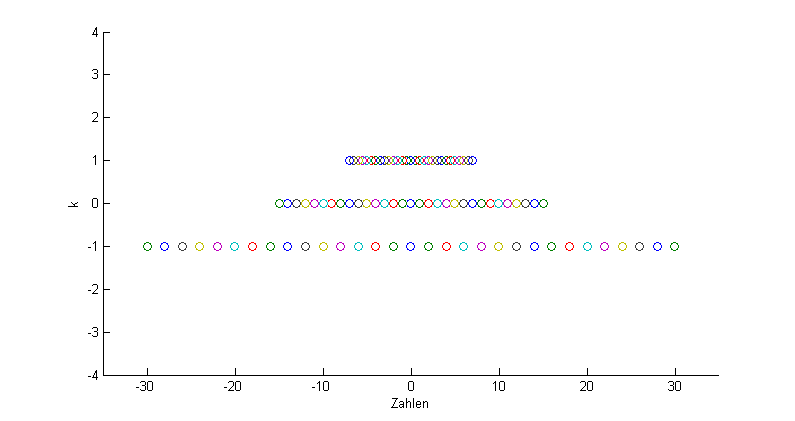
\includegraphics[scale=0.4]{graphiken/fixpunktzahlen-wertebereich.png} 
  \caption{Exakt darstellbare Fixpunktzahlen mit k Nachkommastellen (Entnommen aus \cite{fixpunktzahlen})} \label{img:fixpunktzahlen-wertebereich}
\end{figure} 

Ein weiterer Vorteil von Fixpunktzahlen liegt darin, dass man unter der Verwendung der in \ref{sec:bignum} vorgestellten Big-Nums unendlich viele Nachkommastellen darstellen kann. Aus den
genannten Gründen lässt sich schließen, dass sich die Nutzung von Fixpunktzahlen besser eignet, um $\sqrt{2}$ mit beliebig vielen Nachkommastellen darzustellen. \par

Bei der Division wird ein naives Verfahren verwendet, das im Stile der schriftlichen Division das Ergebnis berechnet und das nur funktioniert, wenn $\text{Dividend} < \text{Divisor}$ gilt. Zu Beginn 
wird der Dividend einmal nach links geshiftet, danach werden in einer Schleife beide Zahlen verglichen. Die Anzahl der Wiederholungen der Schleife entspricht der Anzahl der benötigten Nachkommastellen.
In der i-ten Ausführung der Schleife ergibt sich folgende Fallunterscheidung:
\begin{itemize}
  \item $\text{Dividend} > \text{Divisor}$: Setze das i-te Bit des Ergebnisses auf 1, subtrahiere den Divisor vom Dividenden, shifte den Dividenden einmal nach links
  \item $\text{Dividend} = \text{Divisor}$: Setze das i-te Bit des Ergebnisses auf 1, beende den Algorithmus frühzeitig
  \item $\text{Dividend} < \text{Divisor}$: Setze das i-te Bit des Ergebnisses auf 0, shifte den Dividenden einmal nach links
\end{itemize}

\begin{figure}[h] \centering
  %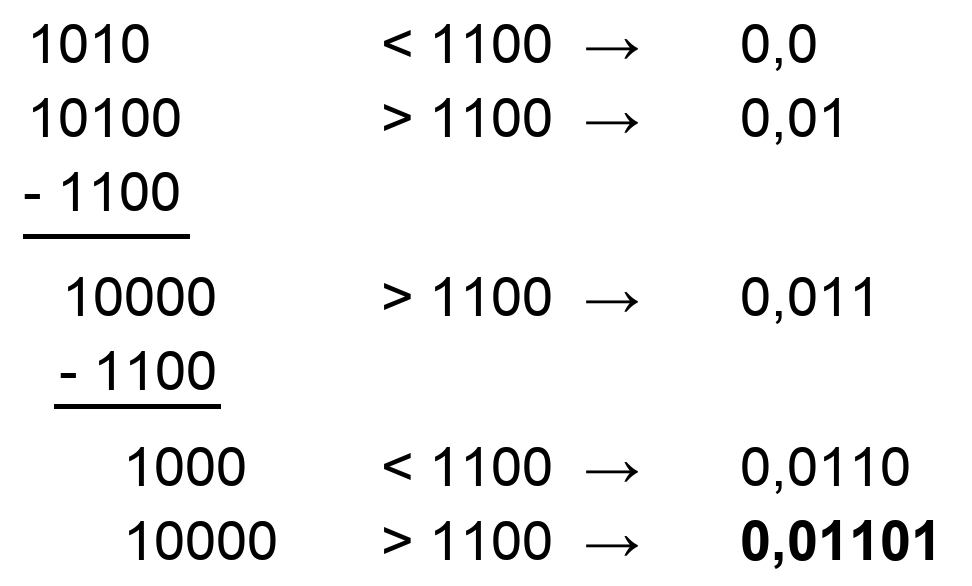
\includegraphics[scale=0.25]{graphiken/division-example.png} 
  \caption{Die einzelnen Rechenschritte zur Berechnung der Division} \label{img:beispiel_division}
\end{figure} 

Als illustratives Beispiel berechnen wir $5_{10} / 12_{10} = (101)_2 / (1100)_2$ mit fünf Nachkommastellen.  
Abbildung \ref{img:beispiel_division} beschreibt das Vorgehen bei der Division. Das Ergebnis ist $(0,01101)_2 = (0,40625)_{10}$. \par
Obwohl dieser Algorithmus zur Kategorie der langsamen Division gehört, bei dem in jedem Schleifendurchlauf nur jeweils eine weitere Nachkommastelle berechnet wird, 
wurde sich explizit dafür entschieden, diesen zu verwenden. Schnelle Divisionsalgorithmen wie die Newton-Raphson-Division können pro 
Schleifendurchlauf die Anzahl der Nachkommastellen zwar verdoppeln \cite{newton_raphson_division}, haben aber aufgrund von wiederholten Multiplikationen und der benötigten initialen Approximation eine schlechtere Performanz, als der hier 
vorgestellte Algorithmus.

% Die Newton-Raphson-Division ist ein Algorithmus zur Berechnung der Division. Er nutzt das Newton-Verfahren, das dafür da ist, Nullstellen von Funktionen zu approximieren und wendet dies so an, um Quotienten zu berechnen. 
% Das Verfahren besteht aus 3 Schritten, die nun erläutert werden \cite{newton_raphson_division}. Wir wollen den Quotienten aus $a$ und $b$ berechen, mit $a, b \in \mathbb{N}$. \\
% Zunächst brauchen wir eine erste Näherung. Wir bitshiften den Quotienten so lange nach rechts, bis $0,5 \leq b < 1,0$. Die erste Näherung erhalten wir mit:
% \begin{equation} \label{eq:erste_naeherung}
%   x_0 = \frac{48}{17} - b \frac{32}{17} \, .
% \end{equation}
%
% Als Nächstes berechnen wir iterativ immer bessere Näherungen:
% \begin{equation} \label{eq:iterationen}
%   x_{i + 1} = x_i (2 - b x_i) \, .
% \end{equation}
% Mit jeder Iteration erhält das Ergebnis doppelt so viele Nachkommastellen wie vorher, es wird auch doppelt so genau. Um die Anzahl der benötigten Iterationen zu erhalten, betrachten wir folgende Formel, wobei k für die erwartete Anzahl an Nachkommastellen im Ergebnis steht:
% \begin{equation} \label{eq:anzahl_iterationen} \text{Iterationen} = \lfloor log_2k\rfloor \, .
% \end{equation}
%
% Um nun das Endergebnis zu erhalten, multiplizieren das Zwischenergebnis mit $a$ und erhalten somit unser Ergebnis der Division.
% Es kann passieren, dass durch die ständige Verdoppelung der Nachkommastellen, die Zahl zu viele davon besitzt als notwendig. Diese Ziffern werden einfach abgeschnitten. \\
% Als illustratives Beispiel berechnen wir $5 / 12$ mit sieben Nachkommastellen. Die Anzahl der Iterationen beträgt $ \lfloor log_27\rfloor = 2$.
% Nach wiederholten bitshiften der Zahl $12$ erhalten wir $(0,1100)_2 = (0,75)_{10}$. Wir berechnen die Zwischenschritte:
% \begin{align}
%   x_0 &= (10,1101.001)_2 - (0,1100)_2 \cdot (1,111)_2 = (1,0110.101)_2 \,; \nonumber \\ 
%   x_1 &= (1,0110.101)_2 \cdot (2_{10} - (0,1100)_2 \cdot (1,0110.101)_2) = (1,0101.0100.0001.0101.00)_2  \,; \nonumber \\
%   x_2 &= (1,0101.0100.0001.0101.00)_2 \cdot (2_{10} - (0,1100)_2 \cdot (1,0101.0100.0001.0101.00)_2) \nonumber \\ 
%       &= (1,0101.0101.0101.0100.0010.1000.1011.0101.0100.0000)_2 \,. \nonumber
% \end{align}
% Multipliziert man $x_2$ mit dem geshifteten $a = (0,0101)_2$ und shiftet dieses so weit, so dass die Zahl nur noch sieben Nachkommastellen besitzt, erhält man das
% Ergebnis $(0,0110.101)_2 = (0,4141)_{10}$, welches sich an der dritten dezimalen Nachkommastelle vom eigentlichen Ergebnis $0,41\overline{6}$ abweicht. \\
 
Wir sind in der Lage, Divisionen durchzuführen und effizient Werte auszurechnen, die das Ergebnis approximieren.

% TODO: Je nach Aufgabenstellung einen der Begriffe wählen
\section{Genauigkeit} \label{sec:genauigkeit}
Wahrscheinlich Genauigkeit, da es die Aufgabe ist, $\sqrt{2}$ beliebig genau darzustellen. \\

Umfangreiche Erklärung darüber, wie die Matrix Elemente an $\sqrt{2}$ konvergiert und Newton-Raphson and die Division. Erklärung, wie die Kombination aus Bignum und Fixkommazahlen unendliche Genauigkeit 
ermöglicht, auf Kosten von Laufzeit, die im nächsten Kapitel beleuchtet wird. \\ 
(1,5 - 2 Seiten?)

\section{Performanzanalyse} \label{sec:performanz}
Im Folgenden werden drei Implementierungen ausgewählt und ihre Performanz verglichen, anschließend erklärt. Die Performanztests wurden auf einem System mit einem Intel i7-9700K Prozessor, 3.60GHz, 16 GB Arbeitsspeicher, 
Ubuntu 20.04, 64 Bit, Linux-Kernel 5.4.0 ausgeführt. Kompiliert wurde mit der Option -03 mit GCC 8.1.0. \par
Die Hauptimplementierung nutzt eine herkömmliche Matrix und alle naiven Implementierungen der Arithmetik von Big-Nums, die erste Vergleichsimplementierung nutzt kompakte Matrizen statt der herkömmlichen. 
Die zweite Vergleichsimplementierung nutzt neben kompakten Matrizen auch die Addition und Subtraktion in SIMD und die Karazuba-Multiplikation. Die Dritte gleicht der zweiten, nur mit dem Unterschied, dass statt der 
Karazuba-Multiplikation eine SIMD Implementierung der Multiplikation verwendet wird. \par

Die Berechnungen wurden mit Eingabegrößen von 1 bis 10000 dezimalen Nachkommastellen jeweils 20 mal durchgeführt und das arithmetische Mittel für jede Eingabegröße wurde in das Diagramm aus Abbildung \ref{img:performanz-diagramm} 
eingetragen.
\begin{figure}[h] \centering
  %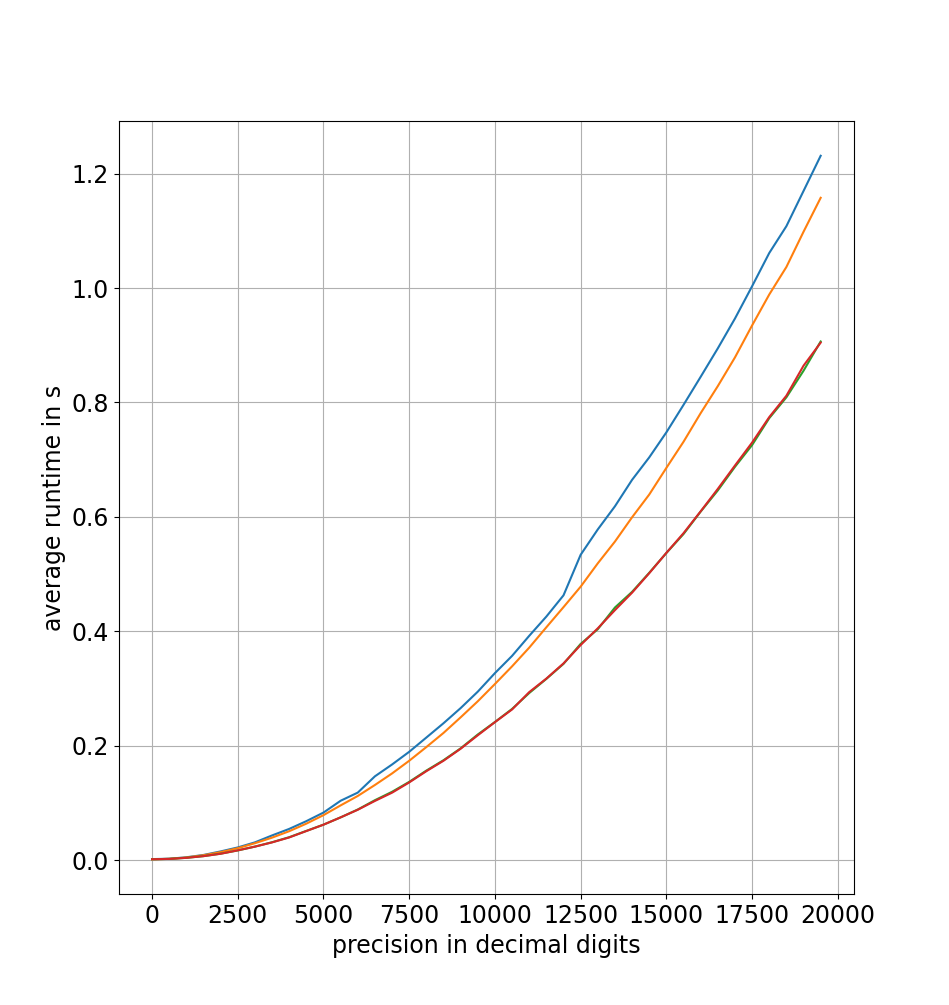
\includegraphics[scale=0.25]{graphiken/performanz-diagramm.jpg} 
  \caption{Performanz der einzelnen Implementierungen} \label{img:performanz-diagramm}
\end{figure} 

An dem Diagramm ist zu erkennen, dass die Hauptimplementierung langsamer ist als die drei Vergleichsimplementierungen. Dies liegt zum Einen an der Tatsache, dass die kompakten Matrizen 4 Multiplikationen einsparen, zum 
Anderen daran, dass die arithmetischen Operationen in SIMD und die Karazuba-Multiplikation schneller sind als die naiven Implementierungen. \par
Aufgrund des nahezu identischen Graphenverlaufs der ersten und der zweiten Vergleichsimplementierung sieht man, dass die Karazuba-Multiplikation und die Multiplikation in SIMD ähnlich performant abschneiden. Dies steht 
entgegen unserer anfänglichen Annahme, dass die Karazuba-Multiplikation wegen ihrer Laufzeit von $\mathcal{O}(n^{1.59})$ schneller ist als die SIMD Multiplikation. Dies kann einige Gründe haben, so ist der Overhead durch die rekursiven 
Funktionsaufrufe ein möglicher Grund. Ein weiterer Aspekt könnte darin liegen, dass die Optimierung durch den Compiler mit der Option -O3 bei der rekursiven Karazuba-Lösung nicht so groß ausfällt.

\section{Zusammenfassung und Ausblick} \label{sec:zusammenfassung}
In dieser Arbeit beschäftigten wir uns mit der Berechnung der Quadratwurzel aus zwei. Es wurden verschiedene Algorithmen thematisiert, wie die Karazuba-Multiplikation oder Divisionsalgorithmus und ihr Einfluss auf die Laufzeit erläutert. Außerdem wurden SIMD Implementierungen berücksichtigt. \par
In einer weiteren Arbeit könnte man daran ansetzen und Big-Num Arithmetiken in AVX implementieren, um weiter die Performanz zu steigern. Des Weiteren könnte man weitere Algorithmen auf die Laufzeit untersuchen und gegebenenfalls implementieren, so zum Beispiel die Goldschmidt-Division. \par
Das Ziel der Arbeit wurde erreicht. Nutzer können, abhängig von ihren Anforderungen oder auch Computerspezifikationen, die Wurzel aus zwei mit beliebigen Nachkommastellen berechnen.

% TODO: Fuegen Sie Ihre Quellen der Datei Ausarbeitung.bib hinzu
% Referenzieren Sie diese dann mit \cite{}.
% Beispiel: CR2 ist ein Register der x86-Architektur~\cite{intel2017man}.
\bibliographystyle{plain}
\bibliography{Ausarbeitung}{}

\end{document}
